\begin{frame}{Les partis politiques en France}
  \footnotesize
  Formez des groupes de 4.
  Chaque groupe va trouver les informations suivantes pour l'un des partis politique français dessous: a) le.s chef.s du parti, b) la position du parti en termes de gauche ou droite et c) les principaux intérêts du parti.
  \begin{columns}
    \column{0.55\textwidth}
      \begin{center}
        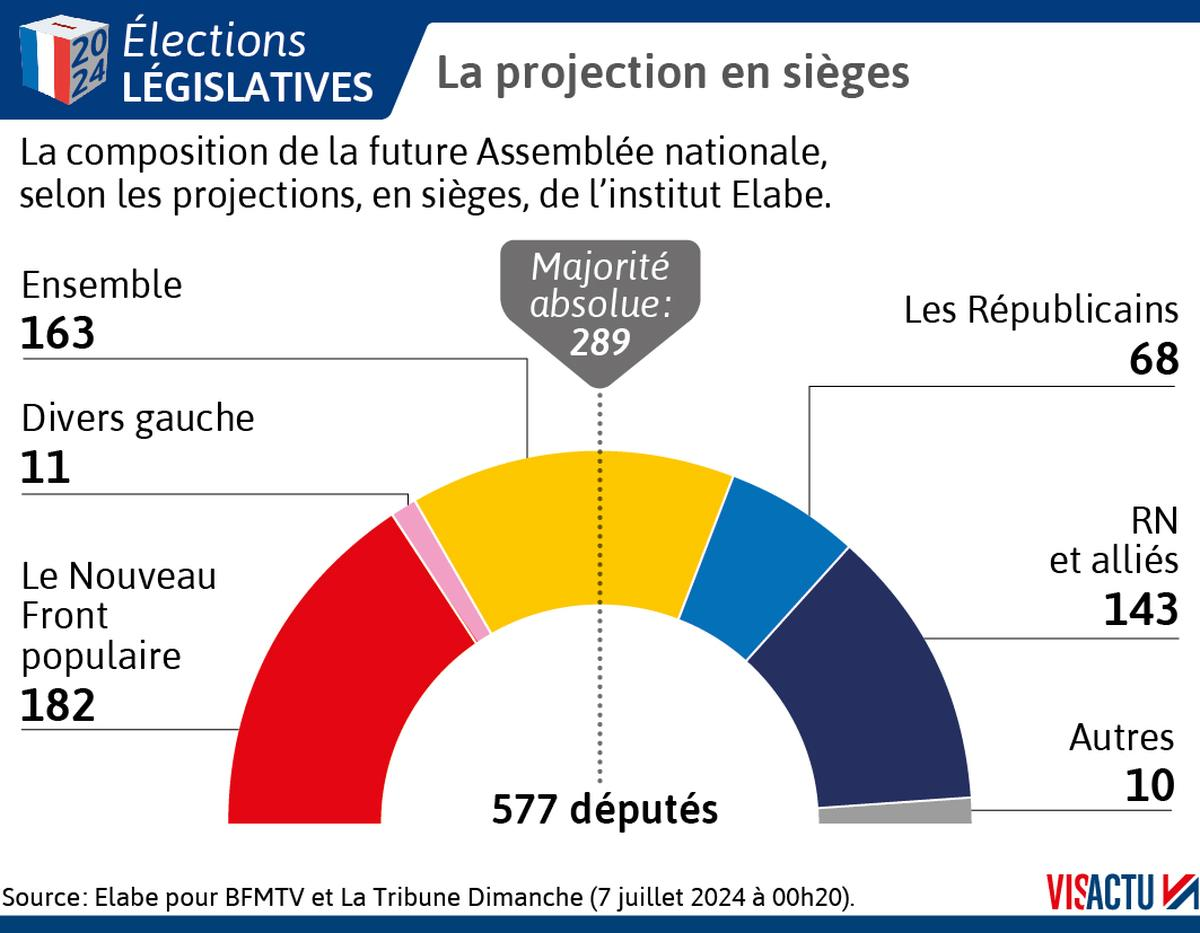
\includegraphics[scale=0.16]{partis_france_2024.jpg}
      \end{center}
    \column{0.45\textwidth}
      \begin{enumerate}
        \item Renaissance (RE) \\ {[Ensemble]}
        \item[] \href{https://parti-renaissance.fr/}{parti-renaissance.fr}
        \item Les Républicains (LR)
        \item[] \href{https://republicains.fr/}{republicains.fr}
        \item La France insoumise (LFI) \\ {[Nouveau front populaire]}
        \item[] \href{https://lafranceinsoumise.fr/}{lafranceinsoumise.fr}
        \item Le Rassemblement national (RN)
        \item[] \href{https://rassemblementnational.fr/}{rassemblementnational.fr}
      \end{enumerate}
  \end{columns}
\end{frame}